\documentclass[letterpaper]{article}
\title{CSE446 Machine Learning, Winter 2015: Homework 1}
\date{Due: Monday, January $28^{th}$, beginning of class}
\usepackage{hyperref}

\usepackage[margin=1in]{geometry}

\usepackage{amsmath,amsfonts}
\usepackage{capt-of}
\usepackage{url}
\usepackage{graphicx}
\usepackage{color}
\usepackage{bbm}
\usepackage{enumerate}
\newcommand{\carlos}[1]{\textcolor{red}{Carlos: #1}}
\newcommand{\field}[1]{\mathbb{#1}} 
\newcommand{\hide}[1]{#1}
\newcommand{\pd}[2]{\frac{\partial #1}{\partial #2}}
\providecommand{\m}[1]{\mathbf{#1}}
\providecommand{\norm}[1]{\left\|#1\right\|}
\providecommand{\sign}[1]{\text{sign}\left(#1\right)}
\DeclareMathOperator*{\argmin}{arg\,min}
\providecommand{\what}{\m{\hat{w}}}
\providecommand{\dw}{\Delta w}
\providecommand{\dmw}{\Delta \m{w}}
\providecommand{\hy}{\hat{y}}
\usepackage[ruled]{algorithm2e}

\begin{document}

\maketitle

\noindent Start Early! Also, typed solutions (specifically those in LaTeX) are preferred to hand-written solutions. Any illegible solutions will be counted wrong at the sole discretion of the grader. Please feel free to use the homework document as a template, putting your solutions inline. Please include your code for Questions 1 and 4.

\section{Decision Trees [32 points]}
For the first two problems, it would be helpful for you to draw the decision boundary of your learned tree in the figure.
\begin{enumerate}
  \item
  \emph{(16 points)} Consider the problem of predicting if a person has a college degree based on
  	age and salary.  The table and graph below contain training data for 10 individuals.
  	
  \begin{center}
  	\begin{tabular}{|c|c|c|}
  	\hline
  	Age & Salary (\$) & College Degree \\
  	\hline
  	24 & 40,000 & Yes \\
  	53 & 52,000 & No \\
  	23 & 25,000 & No \\
  	25 & 77,000 & Yes \\
  	32 & 48,000 & Yes \\
  	52 & 110,000 & Yes \\
  	22 & 38,000 & Yes \\
  	43 & 44,000 & No \\
  	52 & 27,000 & No \\
  	48 & 65,000 & Yes \\
  	\hline
  	\end{tabular}
   \end{center}
   \begin{center}
   	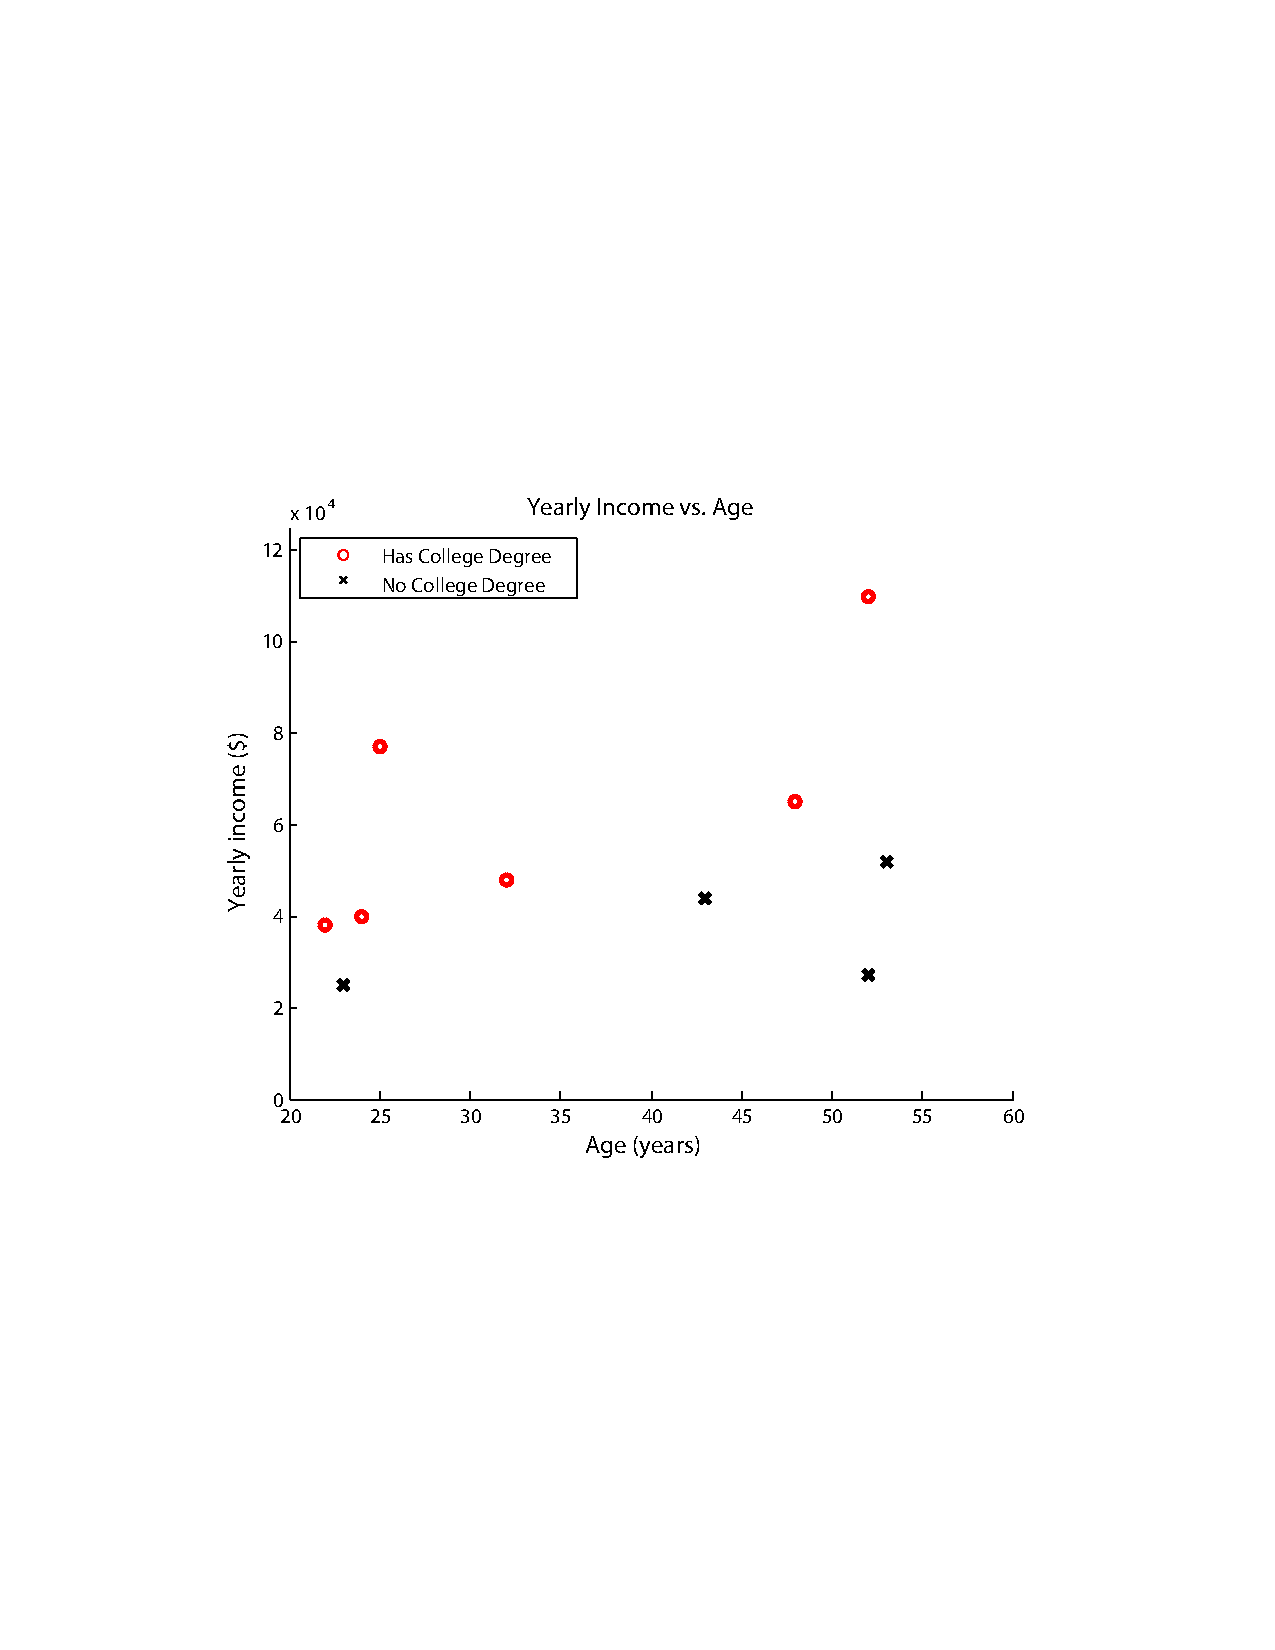
\includegraphics[width=3.5in]{hw1-decision-tree.pdf}
   \end{center}
   Program a decision tree for classifying whether a person has a college degree by greedily choosing threshold splits that maximize
   information gain, as described in class.  
   Draw your tree and include the information gain at each split. How did you decide how to prune your tree?
   Include your code with the submission.  
  \item{(12 points)}
  	A multivariate decision tree is a generalization of univariate decision trees, where more than one attribute
  	can be used in the decision rule for each split.  That is, splits need not be orthogonal to a feature's axis.
  	
  	For the same data, learn a multivariate decision tree where each decision rule is a linear classifier that
  	makes decisions based on the sign of $\alpha x_{age} + \beta x_{income} - 1$.
  	
  	Draw your tree, including the $\alpha, \beta$ and the information gain for each split. Include your code with the submission.
  \item{(4 points)}
  	Multivariate decision trees have practical advantages and disadvantages.  List an advantage and a disadvantage
  	multivariate decision trees have compared to univariate decision trees.
  	 
\end{enumerate}

\section{MLE [20 points]}
This question uses a discrete probability distribution known as the Poisson
distribution. A discrete random variable $X$ follows a Poisson distribution
with parameter $\lambda$ if 

\[
\Pr(X=k)=\frac{\lambda^k}{k!}e^{-\lambda}\qquad
k \in \{0,1,2,\dots\}
\]

\noindent
You are a warrior in Peter Jackson's The Hobbit: Battle of the Five Armies. 
Because Peter decided to make his battle scenes as legendary as possible, 
he's decided that the number of orcs that will die with one swing of your sword is Poisson distributed (i.i.d) with parameter
$\lambda$. You swing your sword eight times in the scene. Later, you go see the movie in theaters
and record the number of orcs slain during each swing of your sword:

\begin{center}
\begin{tabular}{l*{8}{c}r}
Sword Swing         & 1 & 2 & 3 & 4 & 5 & 6 & 7 & 8 \\
\hline
Orcs Slain      & 6 & 4 & 2 & 7 & 5 & 1 & 2 & 5\\
\end{tabular}
\end{center}

\noindent
Let $G=(G_1,\dots,G_n)$ be a random vector where $G_i$ is the number
of orcs slain on swing $i$:

\begin{enumerate}
\item \emph{(6 points)} 
Give the log-likelihood function of $G$ given $\lambda$.
\item \emph{(8 points)} 
Compute the MLE for $\lambda$ in the general case.
\item \emph{(6 point)} 
Compute the MLE for $\lambda$ using the observed $G$.
\end{enumerate}

\section{Regularization Constants [16 points]}
We have discussed the importance of regularization as a technique to avoid
overfitting our models. For linear regression, we could use LASSO
(which uses the $L_1$ norm as a penalty), or ridge regression (which uses
the squared $L_2$ norm as a penalty). In practice, the scaling factor of these
penalties has a significant impact on the behavior of these methods, and must
often be chosen empirically for a particular dataset. In this problem, we look
at what happens when we choose our regularization factor poorly.

For the following, recall that the learning objective under ridge regression is
\[
E_R = \sum_{i=1}^n(y_i - (\hat w_0 + x^{(j)}\hat{w}))^2 + \lambda \| \hat w \|_2^2
\]
where
\begin{equation} \label{eq:ridgepenalty}
\lambda\|\hat w \|_2^2 = \lambda \sum_{i=1}^d (\hat w_i)^2
\end{equation}
and $\lambda$ is our regularization constant.\\

The loss function to be optimized under LASSO regression is
\[
E_L = \sum_{i=1}^n(y_i - (\hat w_0 + x^{(j)}\hat{w}))^2 + \lambda \| \hat w \|_1
\]
where
\begin{equation} \label{eq:lassopenalty}
\lambda \| \hat w \|_1 = \lambda \sum_{i=1}^d |\hat w_i|.
\end{equation}

\begin{enumerate}

\item \emph{(16 points)}
Discuss briefly how choosing too small a $\lambda$ affects the magnitude of
the following quantities.  Please describe the effects for both ridge and
LASSO, or state why the effects will be the same.
\begin{enumerate}
\item The error on the training set.
\item The error on the testing set.
\item The elements of $\hat{w}$.
\item The number of nonzero elements of $\hat{w}$.
\end{enumerate}

\item \emph{(8 points)}
Now discuss briefly how choosing too large a $\lambda$ affects the magnitude
of the same quantities in the previous question.  Again describe the effects
for both ridge and LASSO, or state why the effects will be the same.

\end{enumerate}

\section{Regression, Regularization, and Cross-Validation [40 points]}

Ridge regression is the problem of solving
\begin{equation}\label{eq:ridge}
  \argmin_{\m{w}, w_0} \sum_i{ (\m{X_i} \m{w} + w_0 - \m{y}_i)^2 }
    + \lambda \sum_j \m{w}_j^2 
\end{equation}
Here $\m{X}$ is an $N \times d$ matrix of data, and $\m{X_i}$ is the i-th
row of the matrix. $\m{y}$ is an $N \times 1$ vector of response variables,
$\m{w}$ is a $d$ dimensional weight vector, $w_0$ is a
scalar offset term, and $\lambda$ is a regularization tuning parameter.

\noindent
This question contains two learning objectives, 
\begin{enumerate}
\item Understand the effects of L2 regularization on training and test set errors
\item Use cross-validation to pinpoint the optimal regularization coefficient
\end{enumerate}

\noindent You may use any language for your implementation, but we recommend Python.  Python is a very useful language,
and you should find that Python achieves reasonable enough performance for this problem. You may use common computing packages (such as NumPy or SciPy).
\newline \newline \noindent With the exception of computing objective values or initial conditions, the only matrix operations required
  		are adding vectors, multiplying a vector by a scalar, and computing the dot product between two vectors.
        		Try to use as much vector/matrix computation as possible.

\noindent Finally here are some pointers toward useful parts of Python:
\begin{itemize}
  \item \texttt{numpy}, \texttt{scipy.sparse}, and \texttt{matplotlib} are useful computation packages.
  \item For storing sparse matrices, the \texttt{scipy.sparse.csc\_matrix} (compressed sparse column) format 
  		is fast for column operations.           
  \item Important note for numpy users, \texttt{scipy.sparse.csc\_matrix} uses matrix semantics instead of \texttt{numpy.ndarray} operations.
    Specifically, the * operation is matrix multiplication instead of the elementwise product.
  \item If you're new to Python but experienced with Matlab, consider reading NumPy for Matlab Users
  		at \url{http://wiki.scipy.org/NumPy_for_Matlab_Users}.
\end{itemize}

\noindent This is just our personal advice. We will be able to provide better support for Python users. If you would prefer to use another language, however, that is fine as well.

\noindent Recently Yelp held a recruiting competition on the analytics
website Kaggle.  Check it out at \url{http://www.kaggle.com/c/yelp-recruiting}. 
As a side note, browsing other competitions on the website can give you ideas of some cool applications for machine learning!\\

\noindent For this competition, the task is to predict the number of useful upvotes a particular review will receive. \\

\noindent For many Kaggle competitions (and machine learning methods in general), one of the most important requirements for doing well
is the ability to discover great features.  From an initial list of 1000 features, we have extracted the 100 most relevant for the purpose
of this assignment.

\noindent Yelp provides a variety of data, such as the review's text, date, and restaurant, 
as well as data pertaining to each business, user, and check-ins.  This information has already been
preprocessed for you into the following files:

\begin{center}
\begin{tabular}{l l}
\texttt{upvote\_data\_100.csv} & Data matrix for predicting number of useful votes  \\
\texttt{upvote\_labels.txt} &  List of useful vote counts for each review \\
\texttt{upvote\_features\_100.txt} & Names of each feature for interpreting results \\
\end{tabular}
\end{center}

\noindent For each task, data files contain data matrices, while labels are stored in separate text files. To get you started, the Python following code should load the data:

\begin{verbatim}
import numpy as np
import scipy.sparse as sp

# Load a text file of integers:
y = np.loadtxt("upvote_labels.txt", dtype=np.int)

# Load a text file of strings:
featureNames = open("upvote_features_100.txt").read().splitlines()

# Load a csv of floats:
A = sp.csc_matrix(np.genfromtxt("upvote_data_100.csv", delimiter=","))

\end{verbatim}
\noindent\emph{Note: You don't have to do use a SciPy sparse matrix for this, but it might make your matrix operations far quicker. Also when using the closed-form solution of linear regression, you must include the bias in your training matrix. Add a column of 1's to the front of the matrix}

\noindent For this part of the problem, you have the following tasks:
\begin{enumerate}
  \item \emph{(10 points)} Use the closed-form solution of linear regression to
  predict the number of useful votes a Yelp review will receive.
  Use the first 5000 samples for training, and the remaining 1000 samples for testing. Record the RMSE for your training set and test set.
  
  \item \emph{(10 points)} Now let's look at how regularization changes our training and test set errors.
  Starting at $\lambda = 1$, run ridge regression (using the closed-form solution) on the training set, decreasing $\lambda$ by 25\% 20 times.
  Use 5-fold cross-validation to test for your optimal $\lambda$. For each $\lambda$, record the root-mean-squared-error (RMSE) of the entire training set (all 5000 samples)
  and cross-validation error.
  
  Plot the RMSE values together on a plot against $\lambda$. Which is the optimal $\lambda$? Why? Apply your model using the optimal $\lambda$ on the test set.
  What RMSE value do you obtain?
  		
  \item \emph{(10 points)} Now repeat part 2, using 10-fold cross-validation.
   
  \item \emph{(10 points)} Now split your 5000 training examples into two sets. The first 4000 are your new training set. The final 1000 are a validation set. Repeat part 2 using a validation set as opposed to cross-validation.
  Describe and explain any differences in performance you see when using a validation set vs. k-fold cross-validation.
\end{enumerate}  
\end{document}
